\chapter[Topologická analýza siete \small{(Jakub Novotný)}]{Topologická analýza siete}
Skúmanie globálnej leteckej dopravy vyžaduje prechod od vnímania izolovaných letov k pochopeniu komplexného systému prepojení.
Cieľom tejto kapitoly je formalizovať leteckú sieť ako matematický objekt a následne preskúmať jej topologickú anatómiu – od základnej hustoty
prepojení až po identifikáciu strategických hubov, ktoré držia svetovú konektivitu pohromade.

V našej analýze pracujeme s datasetom obsahujúcim $3214$ letísk (uzlov) a $36907$ pravidelných leteckých spojení (hrán). Skôr než sa zameriame
na konkrétne trasy, musíme pochopiť, aký „tvar“ má táto sieť v abstraktnom grafovom priestore.

\section*{Konštrukcia grafu a metodológia}
Základným kameňom analýzy je definícia orientovaného grafu $G = (V, E)$. Množina vrcholov $V$ reprezentuje jednotlivé letiská, zatiaľ čo orientované
hrany $E \subseteq V \times V$ predstavujú priame letecké linky. Pre výpočtovú efektivitu využívame maticovú reprezentáciu v podobe matice susednosti
$\mathbf{A} \in \mathbb{R}^{3214 \times 3214}$, kde prvok $\mathbf{A}_{i,j}$ nadobúda hodnotu geografickej vzdialenosti medzi letiskami $i$ a $j$.

\section{Globálne charakteristiky a hustota siete}
Prvým zistením pri pohľade na globálnu sieť je jej extrémna riedkosť. Hustota siete, definovaná ako pomer existujúcich hrán k počtu
všetkých možných spojení v kompletnom grafe, dosahuje hodnotu približne $0.00357$.

\begin{equation}
    Hustota = \frac{|E|}{|V|(|V|-1)} \approx 0.357 \%
\end{equation}

Tento výsledok potvrdzuje, že priamočiara dostupnosť medzi ľubovoľnými dvoma letiskami je v globálnom meradle výnimkou, nie pravidlom. Napriek tejto
„riedkosti“ však sieť vykazuje vysokú mieru tranzitivity ($25.01\,\%$). To indikuje, že sieť nie je náhodná, ale je organizovaná do hustých klastrov
– ak existuje spojenie z bodu A do B a z B do C, je $25\%$ šanca, že existuje aj priama linka A $\rightarrow$ C.

\subsection{Komponenty súvislosti a obria komponenta}
Letecký svet v našom modeli nie je dokonale jednotný. Identifikovali sme celkovo $7$ komponentov súvislosti. Avšak analýza ich veľkosti ukazuje na
existenciu tzv. \textbf{Obrieho komponentu} (\textit{Giant Component}), ktorý v sebe pohlcuje až $99.19\,\%$ všetkých letísk ($3188$ uzlov).

Vzhľadom na fakt, že obria komponenta pohlcuje drvivú väčšinu siete, zvyšných $0.81\,\%$ letísk sme pre účely vizualizácie agregovali do súhrnných
geografických bodov. Tento prístup nám umožňuje identifikovať miesta štrukturálnej izolácie bez zbytočného zahltenia mapy detailmi lokálnych
prepojení.

\begin{figure}[H]
    \centering
    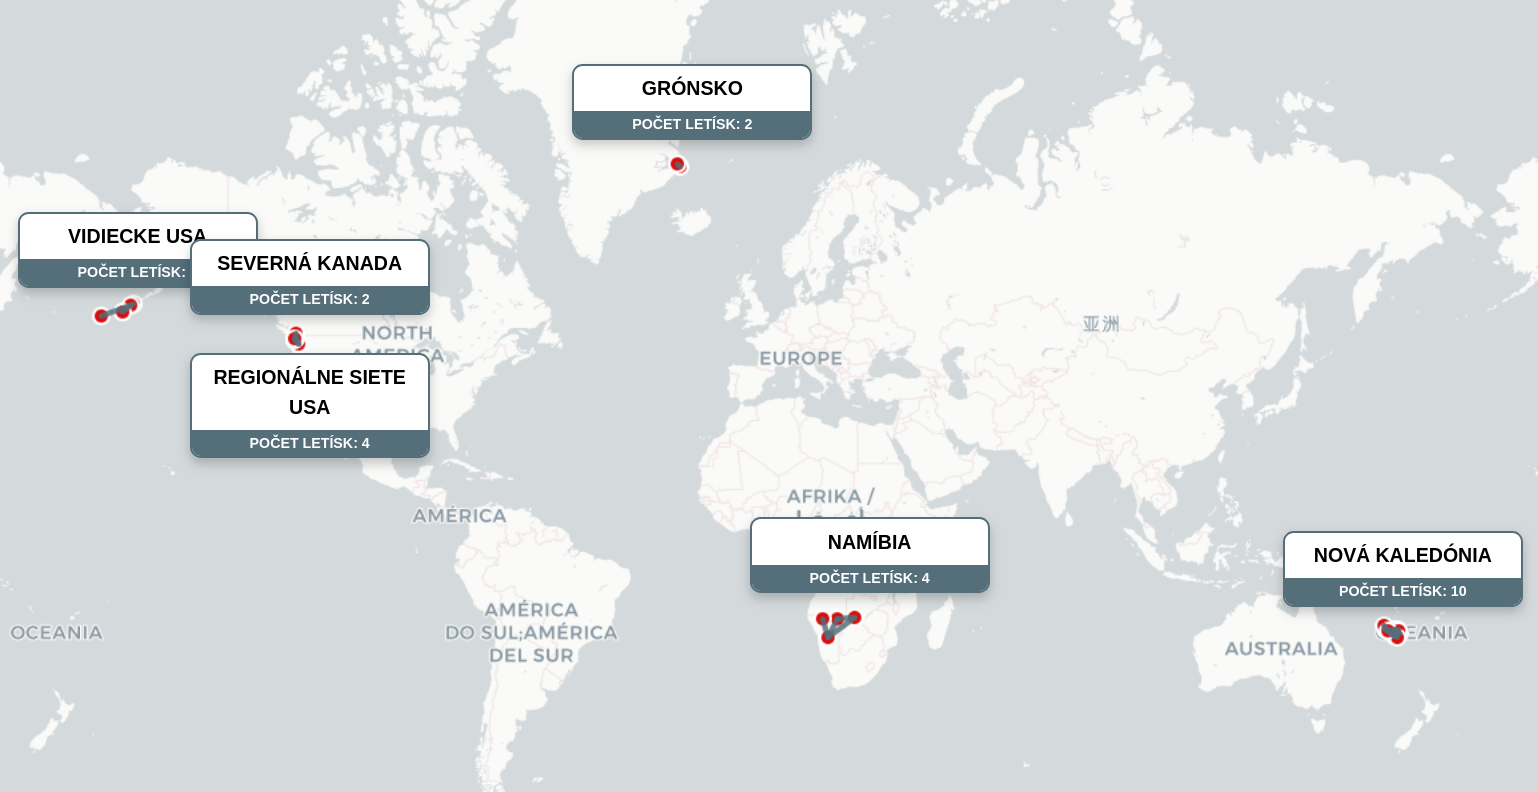
\includegraphics[width=0.9\linewidth]{images/components_map.png}
    \caption{\centering Vizualizácia komponentov (okrem Obrieho komponentu) na mape.}
    \label{fig:islands_map}
\end{figure}


Zistili sme, že izolácia v našom modeli nie je náhodná, ale viaže sa na špecifické geografické celky (Obrázok \ref{fig:islands_map}), ktoré sú v rámci
globálnej logistickej siete odrezané od hlavných hubov. Ide predovšetkým o vnútroštátne siete v \textbf{Namíbii}, \textbf{Grónsku} či špecifické
regionálne okruhy v \textbf{USA} a \textbf{Kanade}. Tieto body predstavujú výzvu pre globálnu integritu siete.

\subsection{Distribúcia stupňov a globálna hierarchia}
\label{sek:stupne}
Kľúčovým indikátorom charakteru reálnej siete je distribúcia stupňov jej vrcholov. Na rozdiel od náhodných grafov, kde majú uzly tendenciu mať podobný
počet susedov, letecká sieť vykazuje extrémnu asymetriu. Priemerný stupeň vrchola v našej sieti je približne $22.97$, avšak medián na úrovni $6$
naznačuje prítomnosť „ťažkého chvosta“ (\textit{heavy-tail}) v rozdelení.

\begin{figure}[H]
    \centering
    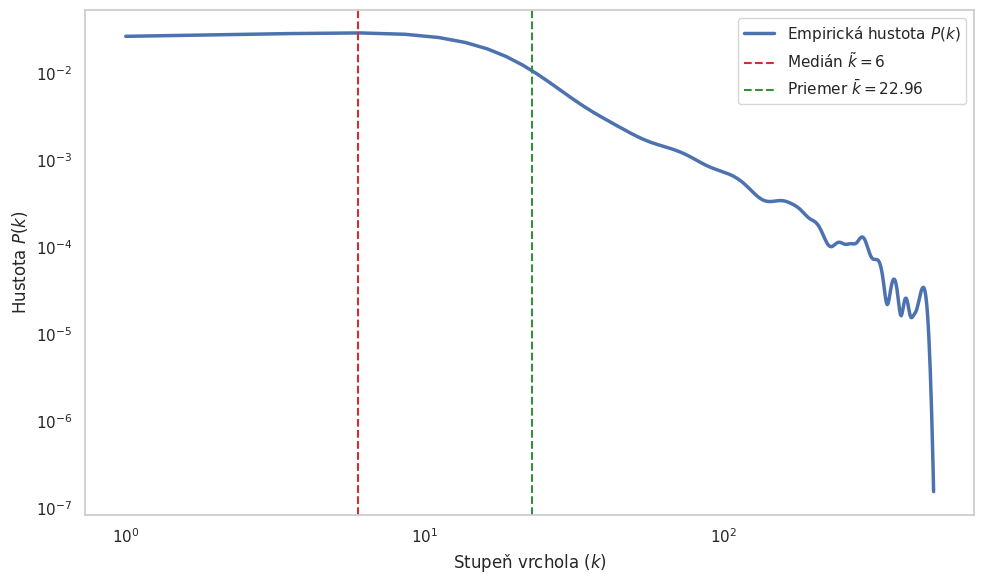
\includegraphics[width=0.7\linewidth]{images/degree_loglog.png}
    \caption{\centering Log-log zobrazenie distribúcie stupňov s KDE odhadom hustoty.}
    \label{fig:degree_dist_analysis}
\end{figure}

V oblasti nízkych stupňov ($k < 10$) je možné pozorovať relatívne stabilnú hustotu (plateau), čo naznačuje, že regionálne letiská s malým počtom
spojení tvoria v systéme robustnú a početne vyrovnanú základňu. Zlom nastáva približne pri stupni $k \approx 20$, odkiaľ distribúcia prechádza do
výrazného poklesu vykazujúceho znaky mocninového zákona.

Tento priebeh s „ťažkým chvostom“ (\textit{heavy-tail distribution}) potvrdzuje prítomnosť hierarchického usporiadania. Zatiaľ čo väčšina uzlov
operuje v režime nízkej konektivity, pravý okraj grafu reprezentuje úzku elitu super-hubov. Extrémna variabilita a oscilácie v záverečnej časti grafu
sú spôsobené nízkou hustotou dát v oblasti najvyšších stupňov, kde sa nachádzajú unikátne uzly ako \textbf{Frankfurt am Main} so stupňom $477$.
Z topologického hľadiska toto rozdelenie indikuje sieť, ktorá je vysoko optimalizovaná na efektívny transport cez centrálne body, hoci za cenu
zvýšenej citlivosti na stabilitu týchto kľúčových uzlov.

\section{Topologická architektúra a komparatívna analýza}

Aby sme odhalili fundamentálne princípy organizácie globálnej leteckej siete, porovnali sme jej vlastnosti s tromi referenčnými nulovými modelmi.
Každý z nich predstavuje inú úroveň náhodnosti a štrukturálnych obmedzení: \textbf{Erdős–Rényiho model} ($G_{ER}$) ako čistú náhodu,
\textbf{Barabási–Albertov model} ($G_{BA}$) ako systém riadený rastom cez huby a \textbf{Konfiguračný model} ($G_{CM}$), ktorý zachováva presnú
hierarchiu (stupne) reálnych uzlov.

\begin{table}[H]
    \centering
    \caption{Komplexné porovnanie sieťových štatistík reálnej siete a teoretických modelov.}
    \label{tab:model_comparison}
    \begin{tabular}{lccc}
        \hline \textbf{Model siete}         & \textbf{Hrany $|E|$} & \textbf{Clustering ($C$)} & 
        \makecell[c]{\textbf{Priem. cesta ($L$)} \\ \small (V Giant Componente)}\\
        \hline \textbf{Reálna letecká sieť} & \textbf{18 859}      & \textbf{0.4918}           & \textbf{2.9585}             \\
        Erdős–Rényi (Náhodný)               & 18 859               & 0.0041                    & 2.5708                      \\
        Barabási–Albert (Huby)              & 18 834               & 0.0201                    & 2.1644                      \\
        Konfiguračný model                  & 17 893               & 0.0732                    & 2.3343                      \\
        \hline
    \end{tabular}
\end{table}

\subsection*{Interpretácia a Small-World fenomén}

Najvýraznejším zistením je prítomnosť \textbf{Small-world efektu}. Tento jav definujeme cez koexistenciu vysokého zhlukovania a krátkych priemerných
vzdialeností. Dosiahnutý index \textbf{$\sigma \approx 108$} (vyjadrujúci pomer clusteringu k dĺžke cesty voči náhode) jasne klasifikuje letectvo ako
vysoko efektívny systém. Pre hlbšiu validáciu sme vypočítali aj Telesfordov koeficient \textbf{$\omega \approx 0.21$} dosadením do následovnej rovnice
\ref{eq:telesford}. Hodnota blízka nule zhora potvrdzuje, že sieť sa nachádza medzi „malým svetom“ a úplným chaosom. 

\begin{equation}
\omega = \frac{L_{rand}}{L} - \frac{C}{C_{latt}}
\label{eq:telesford}
\end{equation}

Kde $C_{latt}$ predstavuje zhlukový koeficient teoretického odhadu pre mriežkovú štruktúru. V praxi to znamená, že napriek obrovským fyzickým
vzdialenostiam žijeme vo „svete štyroch letov“. Priemerná dĺžka cesty $L \approx 2.96$ naznačuje, že globálna dostupnosť je zabezpečená pozoruhodne
malým počtom krokov.

\subsection*{Zaujímavosti a štrukturálne postrehy}

\begin{itemize}
    \item \textbf{Sila komunity vs. Sila hubov:} Konfiguračný model zachováva identickú veľkosť letísk ako realita, no napriek tomu vykazuje takmer
    7-krát nižšie zhlukovanie ($0.073$ vs $0.49$). To dokazuje, že vysoká tranzitivita letectva nie je len vedľajším produktom existencie gigantických
    hubov ako Frankfurt či Atlanta. Je to dôkaz \textbf{geografického determinizmu} — letiská vytvárajú husté lokálne trojuholníky preto, že obsluhujú
    blízke regióny, nie len preto, že sú veľké.

    \item \textbf{Robustnosť „štyroch letov“:} Všimnime si, že priemerná dĺžka cesty $L$ sa naprieč všetkými modelmi (od náhody po realitu) mení len
    minimálne (v rozsahu $2.1$ až $2.9$). To naznačuje, že nízky počet prestupov je \textbf{univerzálnou vlastnosťou} riedkych sietí s daným počtom
    hrán. Realita je však o niečo menej efektívna než náhodné modely, čo je „daň“, ktorú platíme za fyzikálne obmedzenia planéty a nemožnosť spojiť
    každé dve letiská priamou čiarou.

    \item \textbf{Anomália clusteringu:} Hodnota $C = 0.4918$ je v kontexte sieťovej vedy mimoriadne vysoká. Znamená to, že ak máte dve letiská,
    ktoré sú napojené na rovnaký uzol, je takmer $50\,\%$ šanca, že sú prepojené aj medzi sebou. V náhodnom svete by táto šanca bola nižšia než
    $0.5\,\%$. Letecká sieť teda nie je pavučina, ale skôr \textbf{zhluk prepojených ostrovov}.

    \item \textbf{Efektivita BA modelu:} Barabási–Albertov model vykazuje najnižšiu priemernú cestu ($2.16$). To naznačuje, že ak by sa svet riadil
    čistou matematickou optimalizáciou bez ohľadu na štátne hranice a kontinenty, priemerný počet prestupov by klesol o ďalších $20\,\%$.
\end{itemize}

\section{Geografická hierarchia a kontinentálne magistrály}
Topologická štruktúra siete, ktorú sme v predchádzajúcej časti definovali cez vysoký koeficient zhlukovania a nízku priemernú vzdialenosť, získava
jasné kontúry pri pohľade na priestorové rozdelenie dopravy. Naša analýza potvrdzuje, že globálne letectvo nie je homogénnym systémom, ale pozostáva
z masívnych regionálnych podsystémov, ktoré dominujú predovšetkým na severnej pologuli.

\subsection{Vnútrokontinentálna dominancia a lokálne centrá}
Pri skúmaní vnútrokontinentálnej prevádzky (Obrázok \ref{fig:intra_map}) pozorujeme priepastné rozdiely v hustote prepojení medzi svetovými regiónmi.
Severná pologuľa funguje ako motor globálnej konektivity, kde \textbf{Ázia (18 004 prepojení)}, \textbf{Európa (16 597)} a
\textbf{Severná Amerika (15 844)} tvoria takmer uzavreté a vysoko redundantné ekosystémy. Tieto čísla ostro kontrastujú s južnou pologuľou a Afrikou,
kde celková konektivita kontinentov dosahuje len zlomok týchto hodnôt, napríklad v prípade \textbf{Afriky (2 104)} alebo \textbf{Oceánie (1 654)}.

V rámci týchto geografických segmentov dopravy identifikujeme kľúčové uzly, ktoré fungujú ako primárne lokálne distributéry tokov. Absolútnym lídrom
v počte vnútorných prepojení je \textbf{Atlanta (1 695)}, ktorá v našom modeli dominuje severoamerickému trhu. V Ázii túto rolu zastáva
\textbf{Peking (851)} a \textbf{Šanghaj (680)}, zatiaľ čo v Európe sa do popredia dostáva \textbf{Barcelona (646)} a \textbf{Palma de Mallorca (544)}.
Práve prítomnosť takto silných regionálnych uzlov naznačuje, že sieť je formovaná nielen biznisovými centrami, ale aj silnými turistickými tokmi.
Tieto lokálne huby sú priamo zodpovedné za vysokú nameranú tranzitivitu, nakoľko vytvárajú extrémne husté lokálne susedstvá, kde je väčšina
regionálnych destinácií dostupná na jeden prestup.

\begin{figure}[H]
    \centering
    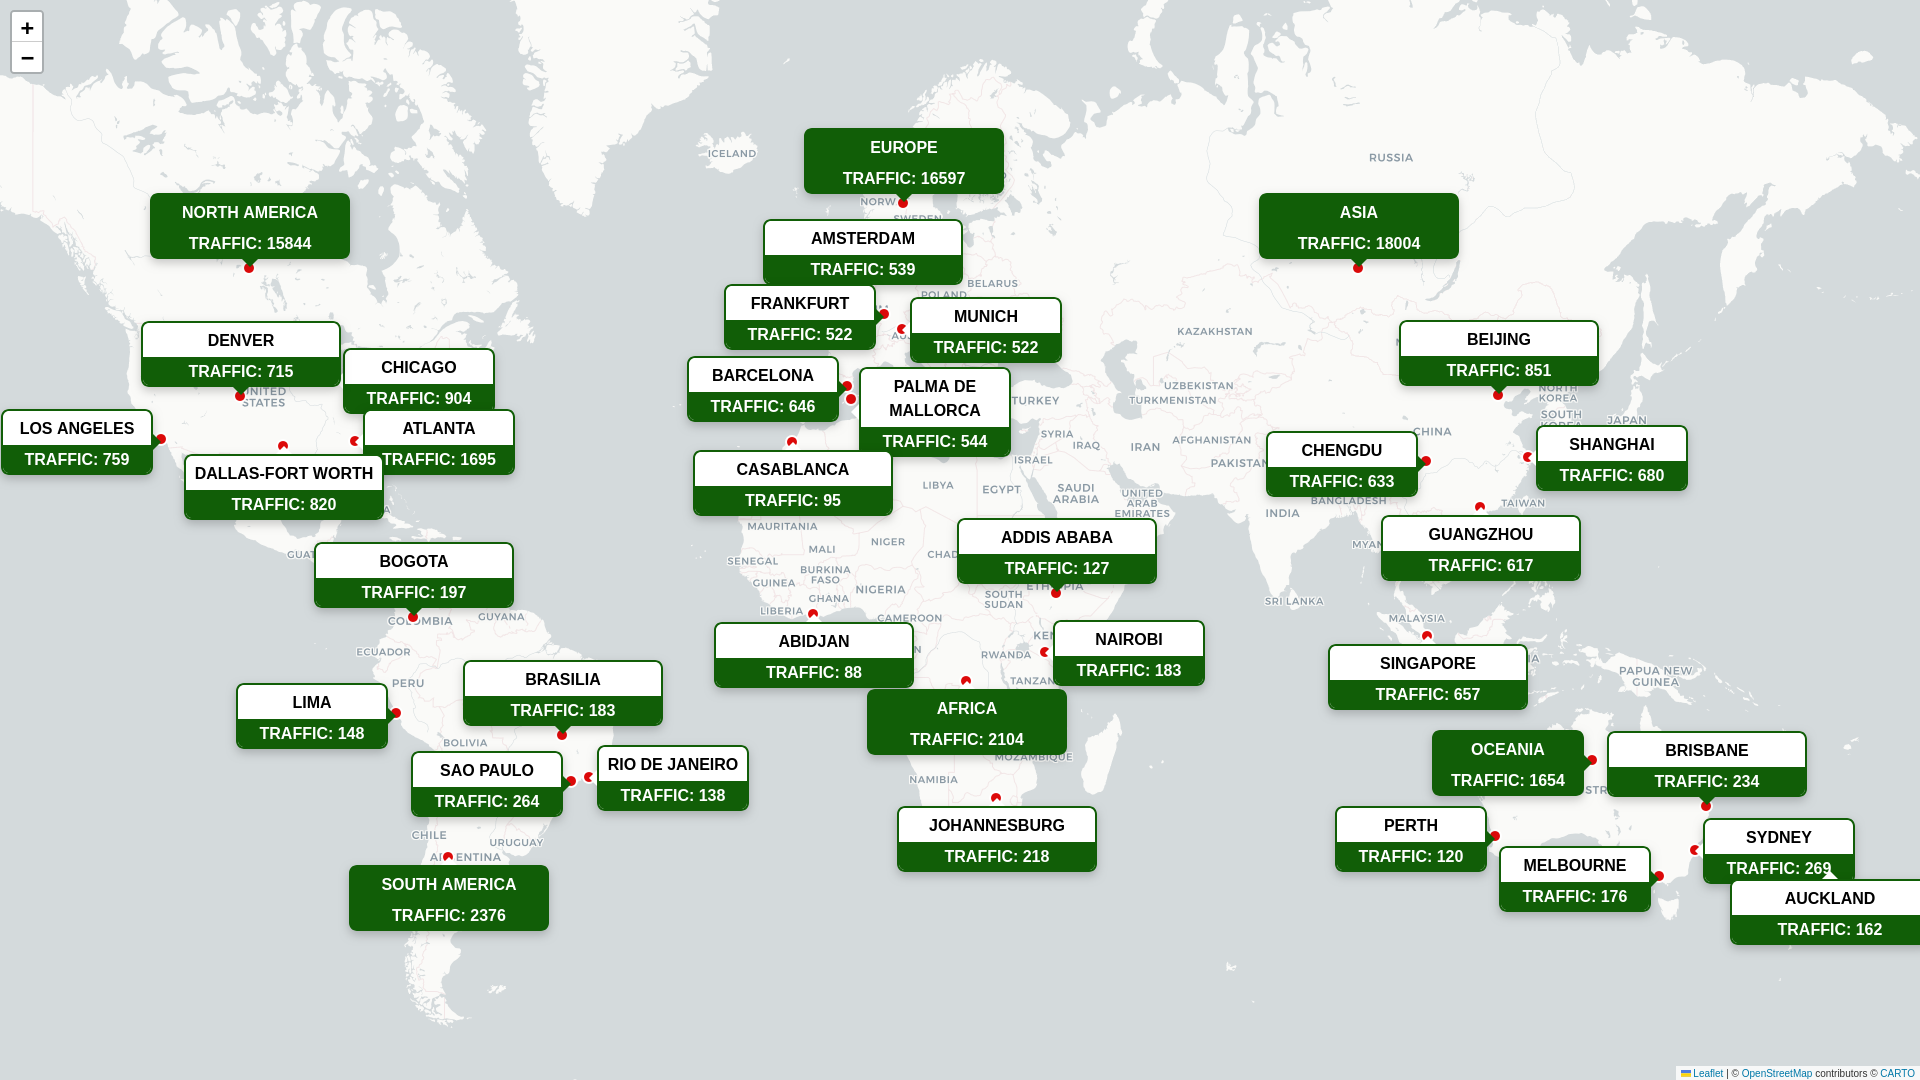
\includegraphics[width=0.95\textwidth]{images/incontinental.png}
    \caption{Vizualizácia vnútrokontinentálnej dopravy a kľúčových regionálnych hubov.}
    \label{fig:intra_map}
\end{figure}

\subsection{Interkontinentálne magistrály: Mosty medzi svetmi}

Zatiaľ čo tisíce lokálnych letov vytvárajú stabilitu a hustotu vnútri regiónov, globálnu integritu celého systému držia pohromade strategické
interkontinentálne toky (Obrázok \ref{fig:inter_map}). Týchto $28$ hlavných magistrál funguje ako topologické „skratky“. Tie sú v konečnom dôsledku
zodpovedné za nízku priemernú dĺžku cesty naprieč planétou, pretože bez nich by sa sieť rozpadla na súbor navzájom izolovaných komponentov.

Z vizualizácie tokov vyplývajú tri hlavné piliere globálnej konektivity. Absolútne dominantnou osou je \textbf{Euro-Ázijské prepojenie
(1 837 unikátnych trás)}, ktoré predstavuje najmohutnejší medzikontinentálny tok v celom systéme a slúži ako faktická chrbtica svetovej dopravy.
Druhým pilierom je \textbf{Transatlantický most (1 001 trás)} spájajúci Európu so Severnou Amerikou. Tieto dve osi potvrdzujú strategické postavenie
Európy ako centrálneho dispečera, ktorý vďaka svojej geografickej polohe integruje východnú a západnú pologuľu do jedného celku.

\begin{figure}[H]
    \centering
    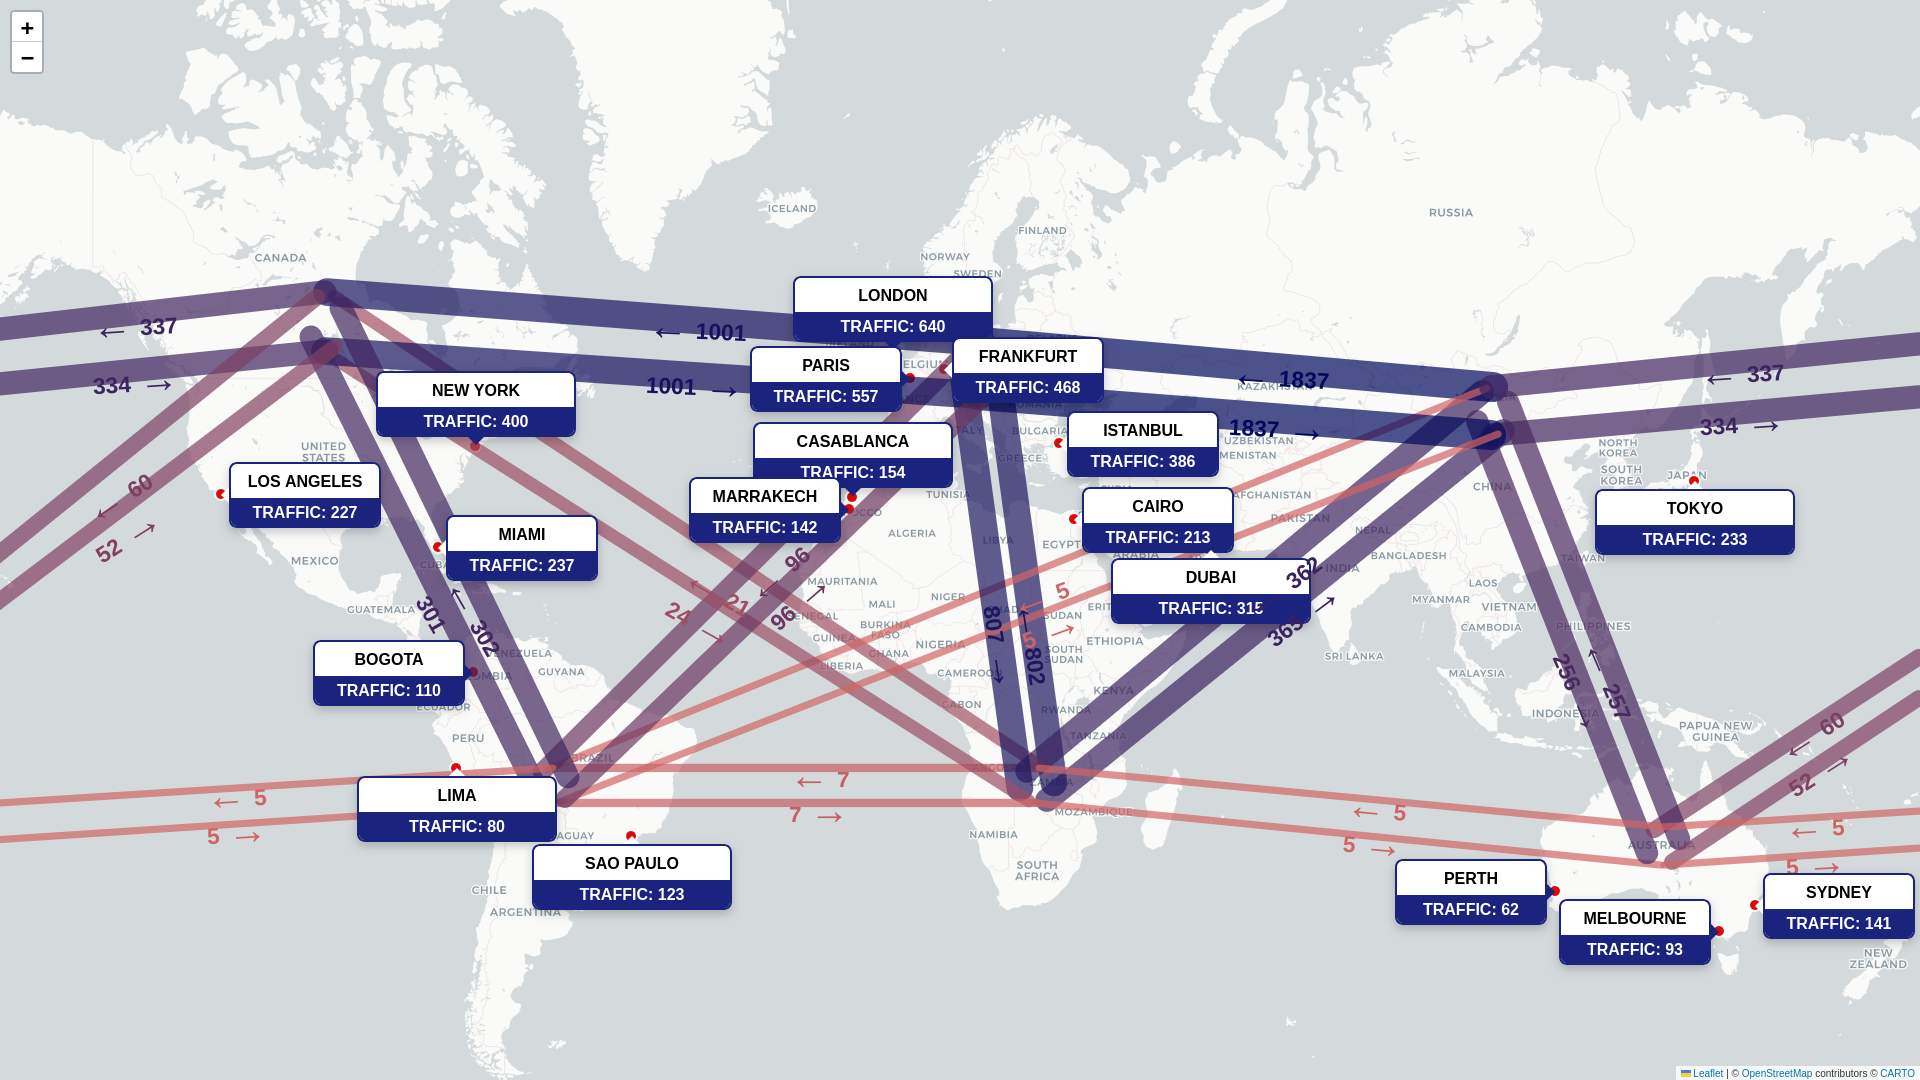
\includegraphics[width=0.95\textwidth]{images/intercontinental_map.png}
    \caption{Vizualizácia hlavných interkontinentálnych tokov a globálnych magistrál.}
    \label{fig:inter_map}
\end{figure}

Zaujímavým prvkom je vertikálna integrácia \textbf{Afriky}, ktorá je v súčasnosti silne naviazaná primárne na Európu (viac než 800 trás cez huby ako
Casablanca či Káhira), no vykazuje minimálnu priamu konektivitu s Južnou Amerikou či Oceániou. Tento stav naznačuje, že globálna sieť je prísne
hierarchická. Zatiaľ čo severné kontinenty sú prepojené robustnými „multivláknovými“ mostami, južné kontinenty sa spoliehajú na obmedzený počet
strategických trás prechádzajúcich cez globálne huby. Práve táto vysoká koncentrácia tokov do niekoľkých kľúčových kanálov vysvetľuje, prečo je
sieť síce topologicky efektívna (\textit{Small-world}), ale zároveň potenciálne zraniteľná voči cieleným výpadkom v hlavných tranzitných regiónoch.